\documentclass[12pt,letter]{article}
\usepackage[moduleName=FME7]{KautenjaDSP}
% import a debugging package to show the margin boxes
% \usepackage{showframe}
% set the graphics path to the img directory
\graphicspath{{img/}}

% algorithm2e stuff
% \SetKwInOut{Objects}{$\CKmatrix{O}$}
% \SetKwInOut{Weights}{$\CKvector{w}$}

\begin{document}
\titlePage{FME7-Logo}{FME7-Module}{KautenjaDSP}

% -------------------
% MARK: Overview
% -------------------

\section{Overview}

FME7 is an emulation of the SunSoft FME7 (5B) sound chip from the Nintendo Entertainment System (NES) for VCV Rack. The FME7 chip contains three pulse wave generators with level control.

FME7 provides the key features of the FME7 chip, namely,
\begin{itemize}
  \item \textbf{Triple pulse wave generator:} Triple 12-bit pulse waveform generator with duty cycle of $50\%$
  \item \textbf{Amplitude modulation:} Manual and CV control over the individual voice levels
\end{itemize}

% -------------------
% MARK: Panel Layout
% -------------------

\clearpage
\section{Panel Layout}

\begin{figure}[!htp]
\centering
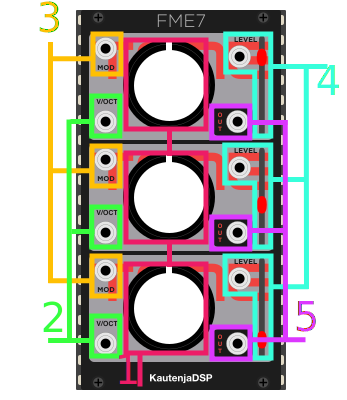
\includegraphics{FME7-Manual}
\end{figure}

\begin{enumerate}
  \item Coarse frequency control for the pulse A, B, and C waveform generators.
  \item $V$/Octave inputs for pulse A, B, and C waveform generators.
  \item linear CV frequency modulation for pulse A, B, and C waveform generators.
  \item Level control for pulse A, B, and C waveform generators. When no input is connected, the slider controls the level from $0\%$ to $100\%$. When an input is connected, the slider acts as an attenuator.
  \item Channel outputs, ${\approx}10V_{pp}$.
\end{enumerate}

% -------------------
% MARK: References
% -------------------

\clearpage
\renewcommand\refname{References \& Acknowledgments}
\nocite{*}
\bibliographystyle{apalike}
\bibliography{references}

\end{document}
